\documentclass[tikz,border=1mm]{standalone}
\usetikzlibrary{fit,shapes.geometric,arrows}

\begin{document}
	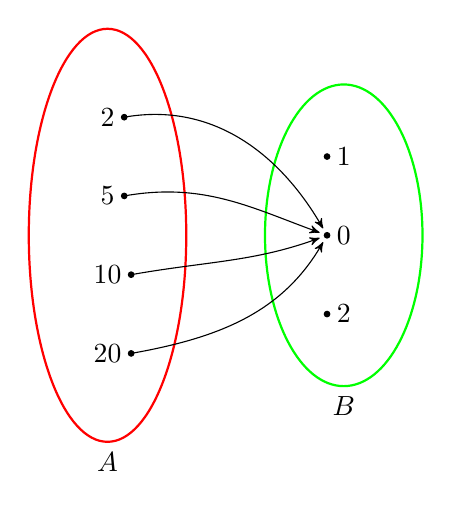
\begin{tikzpicture}
	\node (2) at (0,0) {2};\filldraw(2.east) circle (1pt);
	\node (5) [below of=2] {5};\filldraw(5.east) circle (1pt);
	\node (10) [below of=5] {10};\filldraw(10.east) circle (1pt);
	\node (20) [below of=10] {20};\filldraw(20.east) circle (1pt);
	\node[fit=(2) (5) (10) (20), ellipse, draw=red, minimum width=2cm, thick, label=below:\(A\)]{};
	
	\node (1) at (3,-0.5) {1};\filldraw(1.west) circle (1pt);
	\node (0) [below of=1] {0};\filldraw(0.west) circle (1pt);
	\node (2_2) [below of=0] {2};\filldraw(2_2.west) circle (1pt);
	\node[fit=(1) (0) (2_2), ellipse, draw=green, minimum width=2cm,thick, label=below:\(B\)]{};
	
	\draw[->, shorten >=.1cm,>=stealth'] (2.east) to [out=10, in=120] (0.west);
	\draw[->, shorten >=.1cm,>=stealth'] (5.east) to [out=10, in=160] (0.west);
	\draw[->, shorten >=.1cm,>=stealth'] (10.east) to [out=10, in=200] (0.west);
	\draw[->, shorten >=.1cm,>=stealth'] (20.east) to [out=10, in=240] (0.west);
	\end{tikzpicture}
\end{document}